%%******************************************************************************
%%
%% Metodologia.tex
%%
%%******************************************************************************
%%
%% Title......: Introduction
%%
%% Author.....: GSCAR-DFKI
%%
%% Started....: Nov 2013
%%
%% Emails.....: elael@poli.ufrj.br
%%
%% Address....: Universidade Federal do Rio de Janeiro
%%              Caixa Postal 68.504, CEP: 21.945-970
%%              Rio de Janeiro, RJ - Brasil.
%%
%%******************************************************************************


%%******************************************************************************
%% SECTION - Anexo
%%******************************************************************************


\section{Datasheets}
\subsection{Encoder}
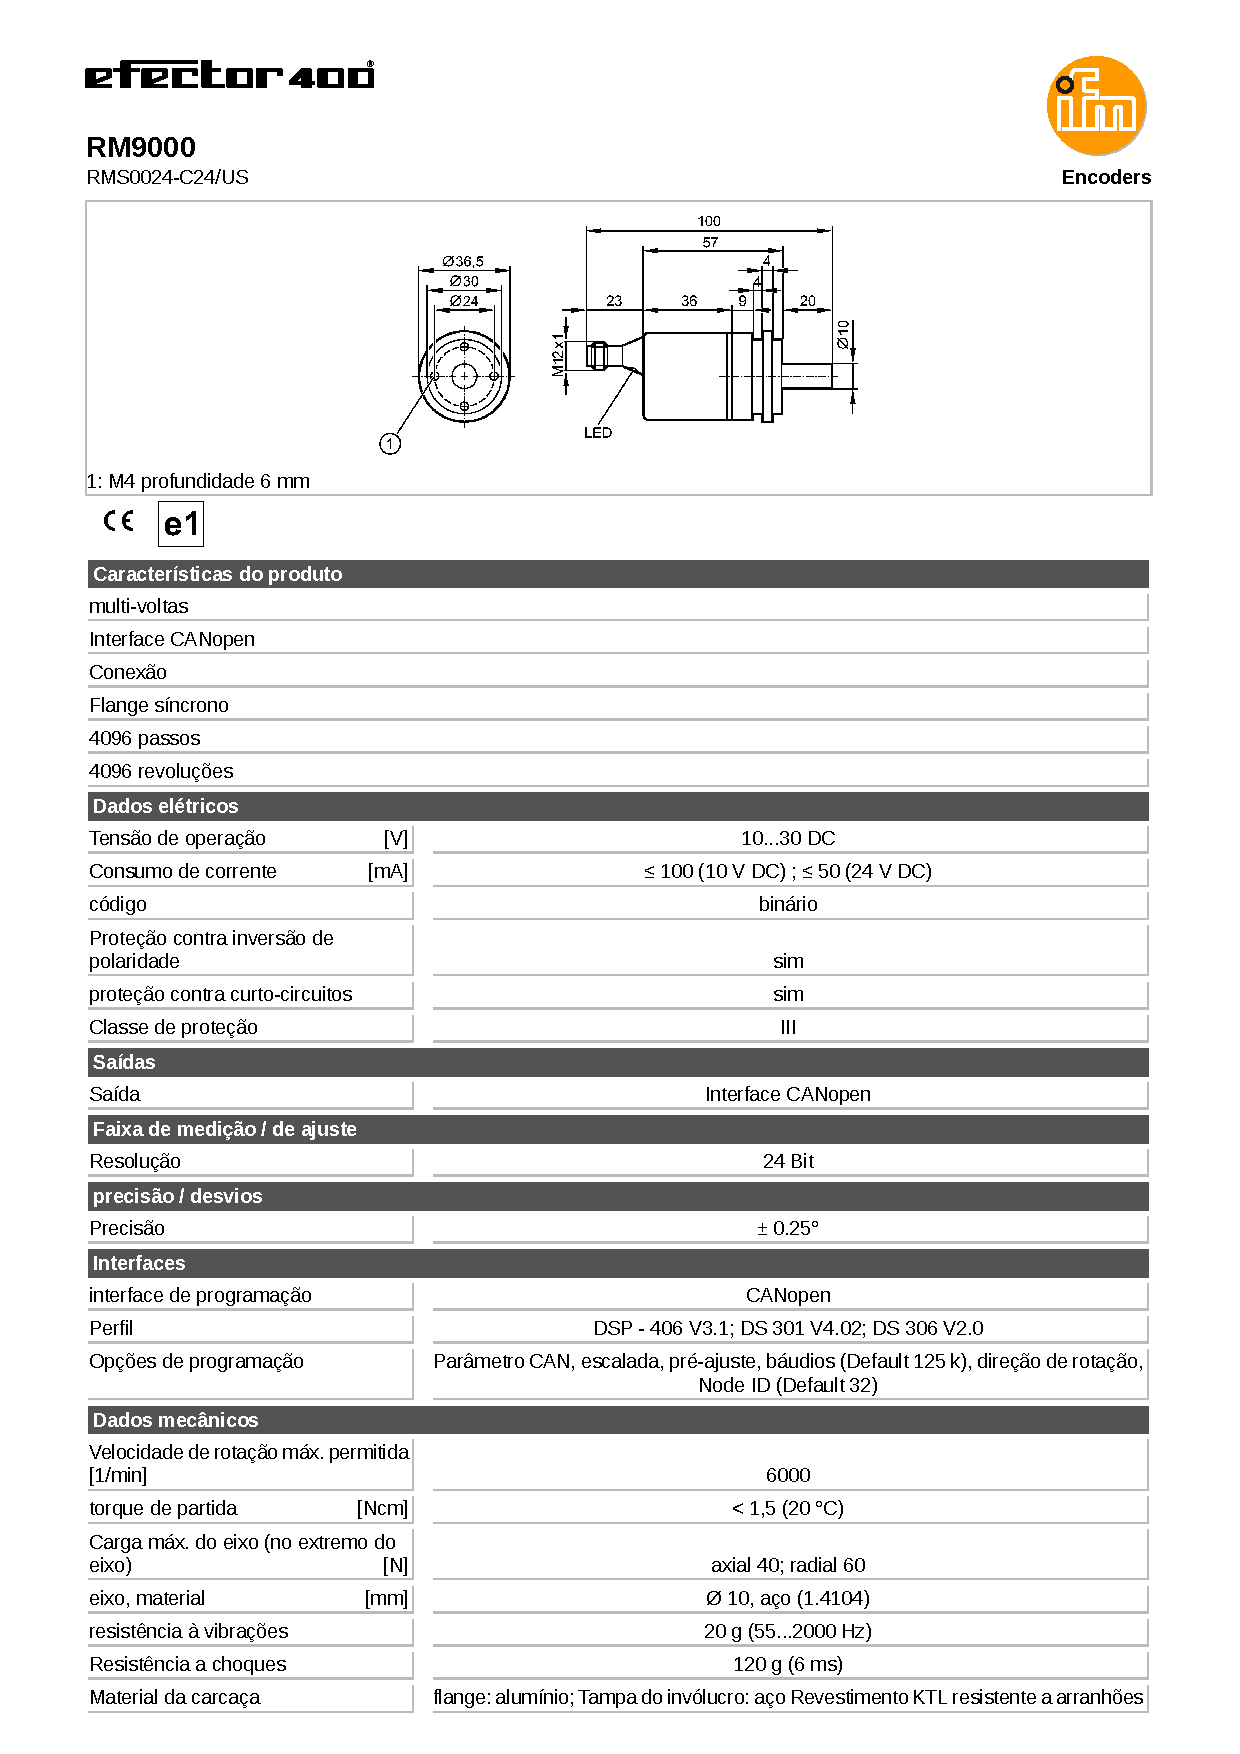
\includegraphics[width=1\columnwidth]{figs/datasheets/rm9000.pdf}
\includepdf[pages={2-},width=1\columnwidth,pagecommand=\thispagestyle{plain}]{figs/datasheets/rm9000.pdf}
\subsection{Sonar}
\includegraphics[width=1\columnwidth, page=2]{figs/datasheets/sonar.pdf}
\subsection{Pan \& Tilt}
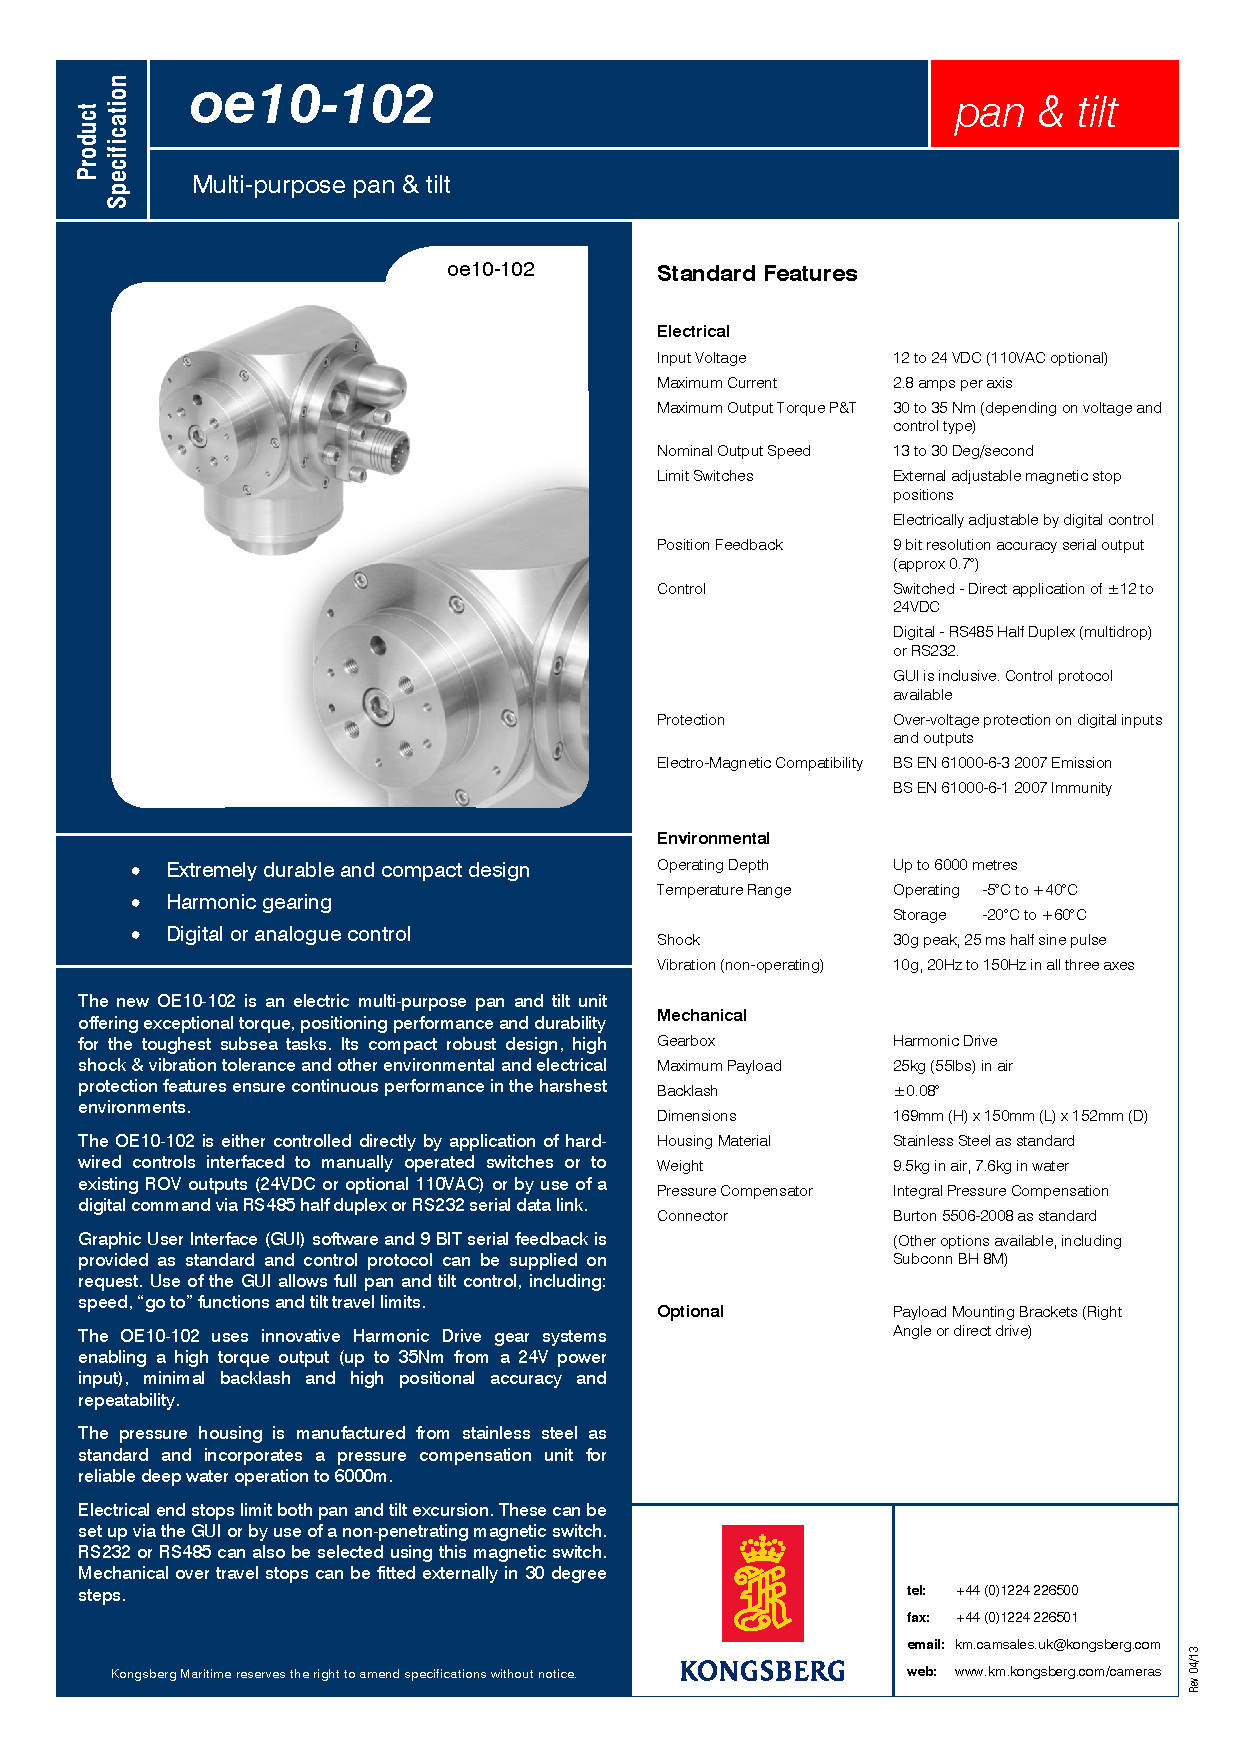
\includegraphics[width=1\columnwidth]{figs/datasheets/pantilt.pdf}
\subsection{Sensor Indutivo}
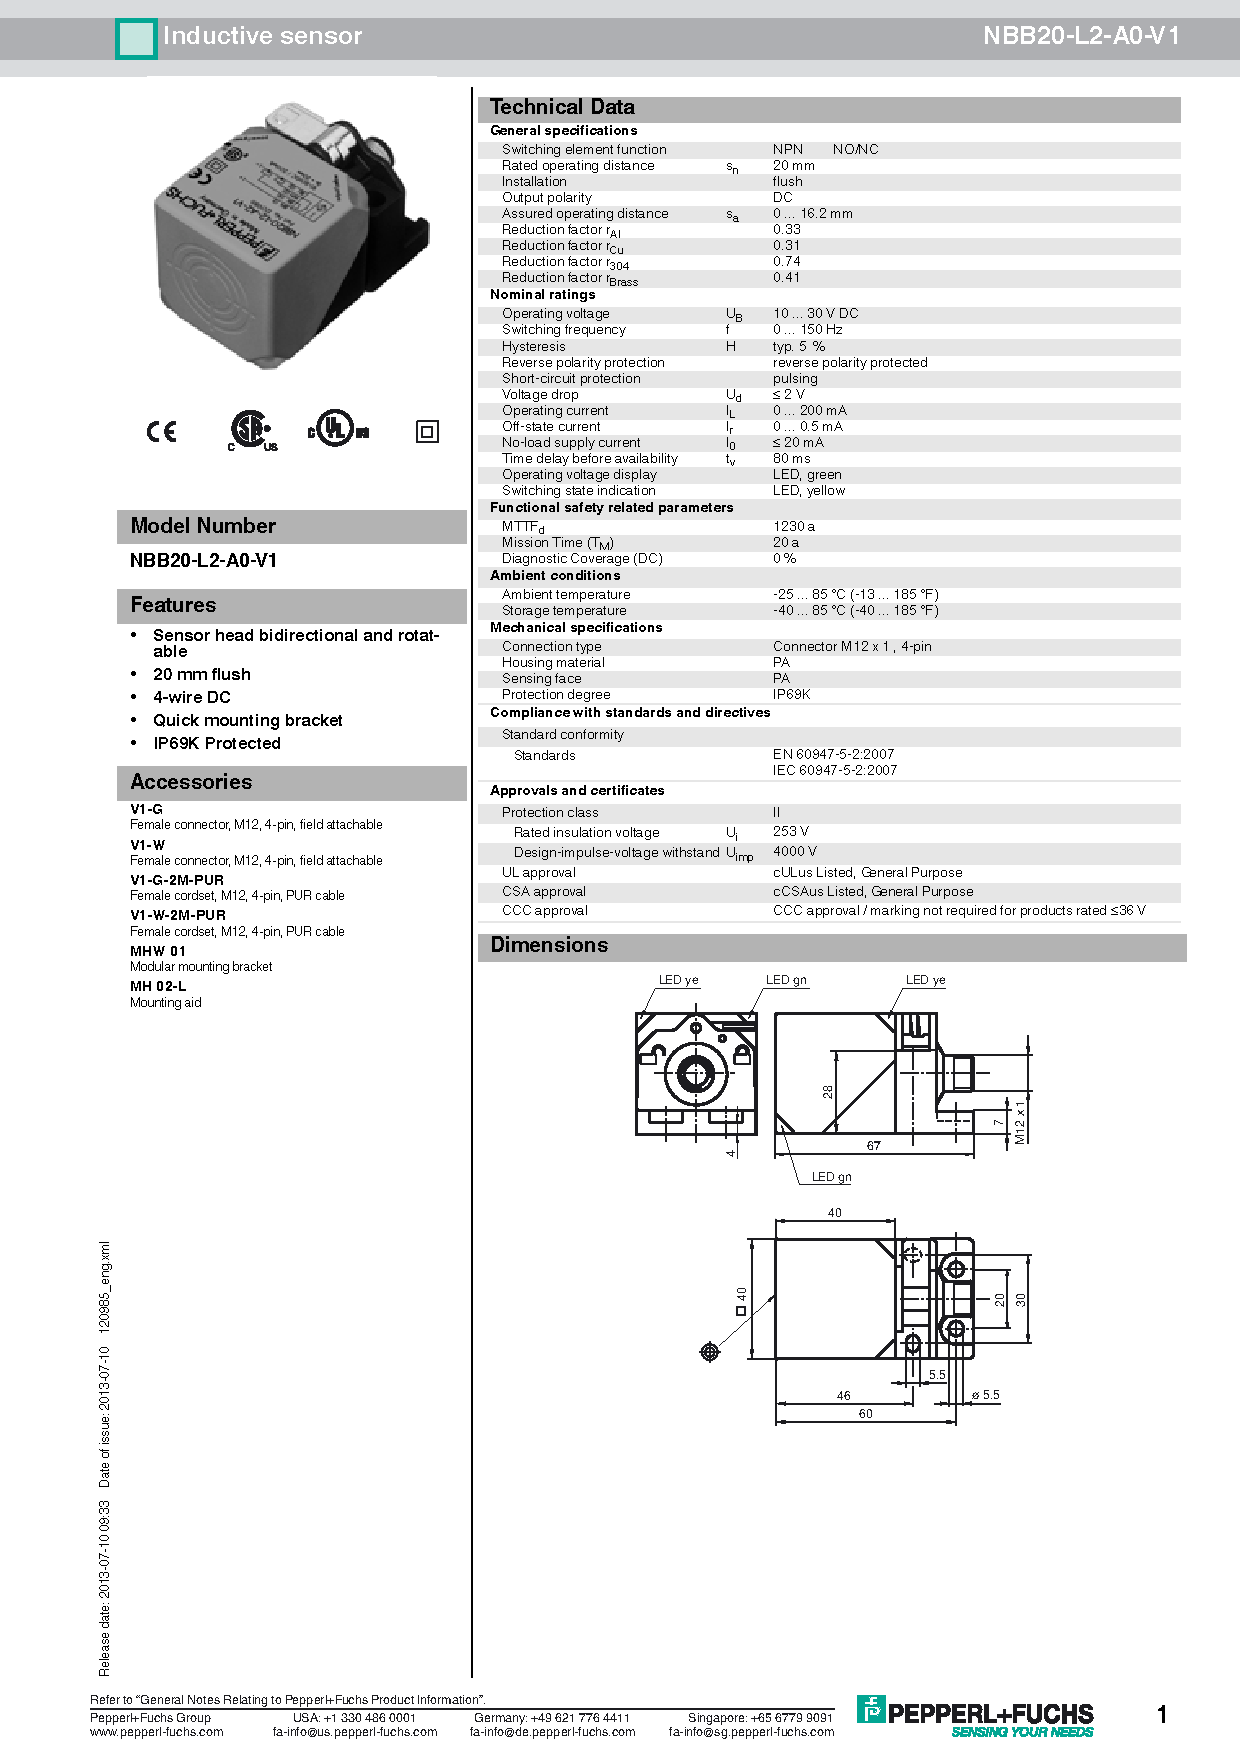
\includegraphics[width=1\columnwidth]{figs/datasheets/inductive.pdf}
\includepdf[pages={2-},width=1\columnwidth,pagecommand=\thispagestyle{plain}]{figs/datasheets/inductive.pdf}
\subsection{Sensor de inclinação}
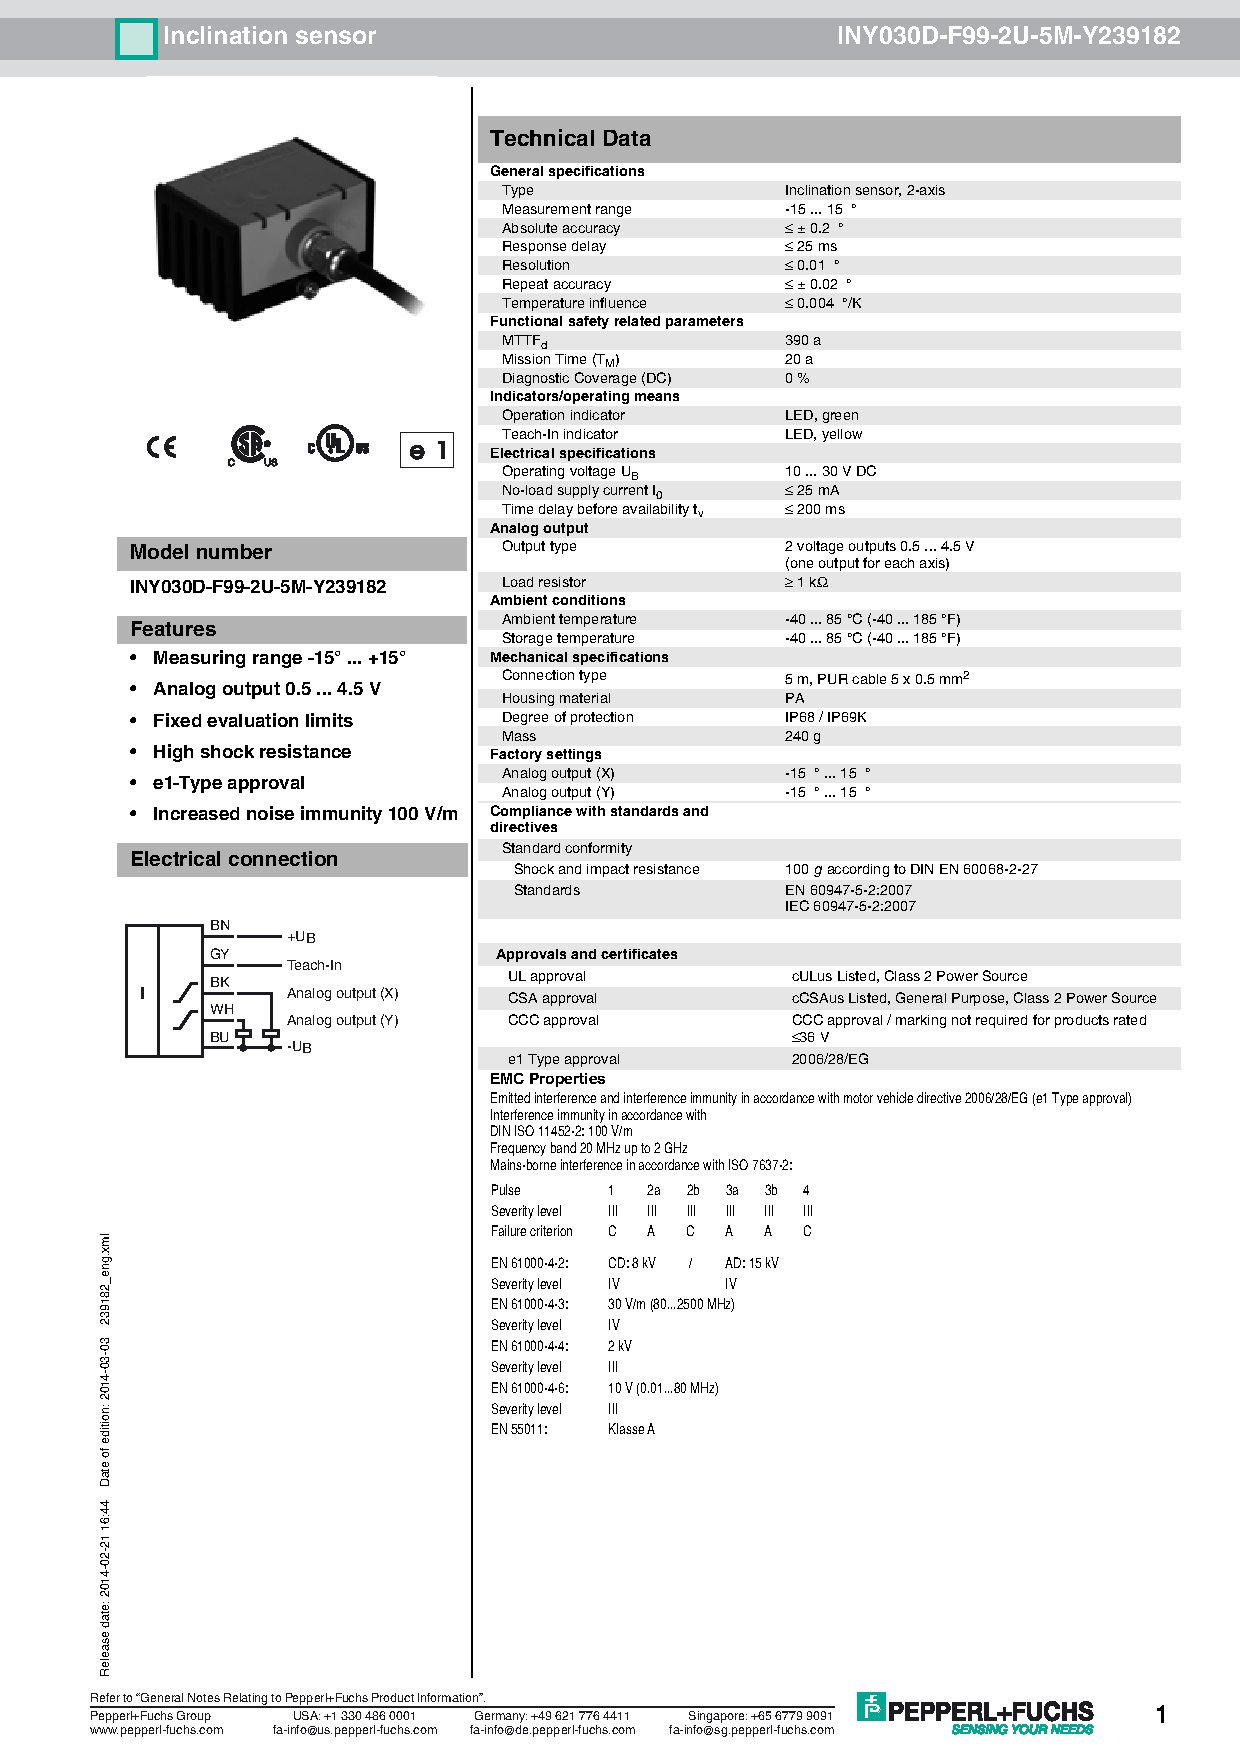
\includegraphics[width=1\columnwidth]{figs/datasheets/inclinacao.pdf}
\includepdf[pages={2-},width=1\columnwidth,pagecommand=\thispagestyle{plain}]{figs/datasheets/inclinacao.pdf}
\subsection{Sensor de Pressão}
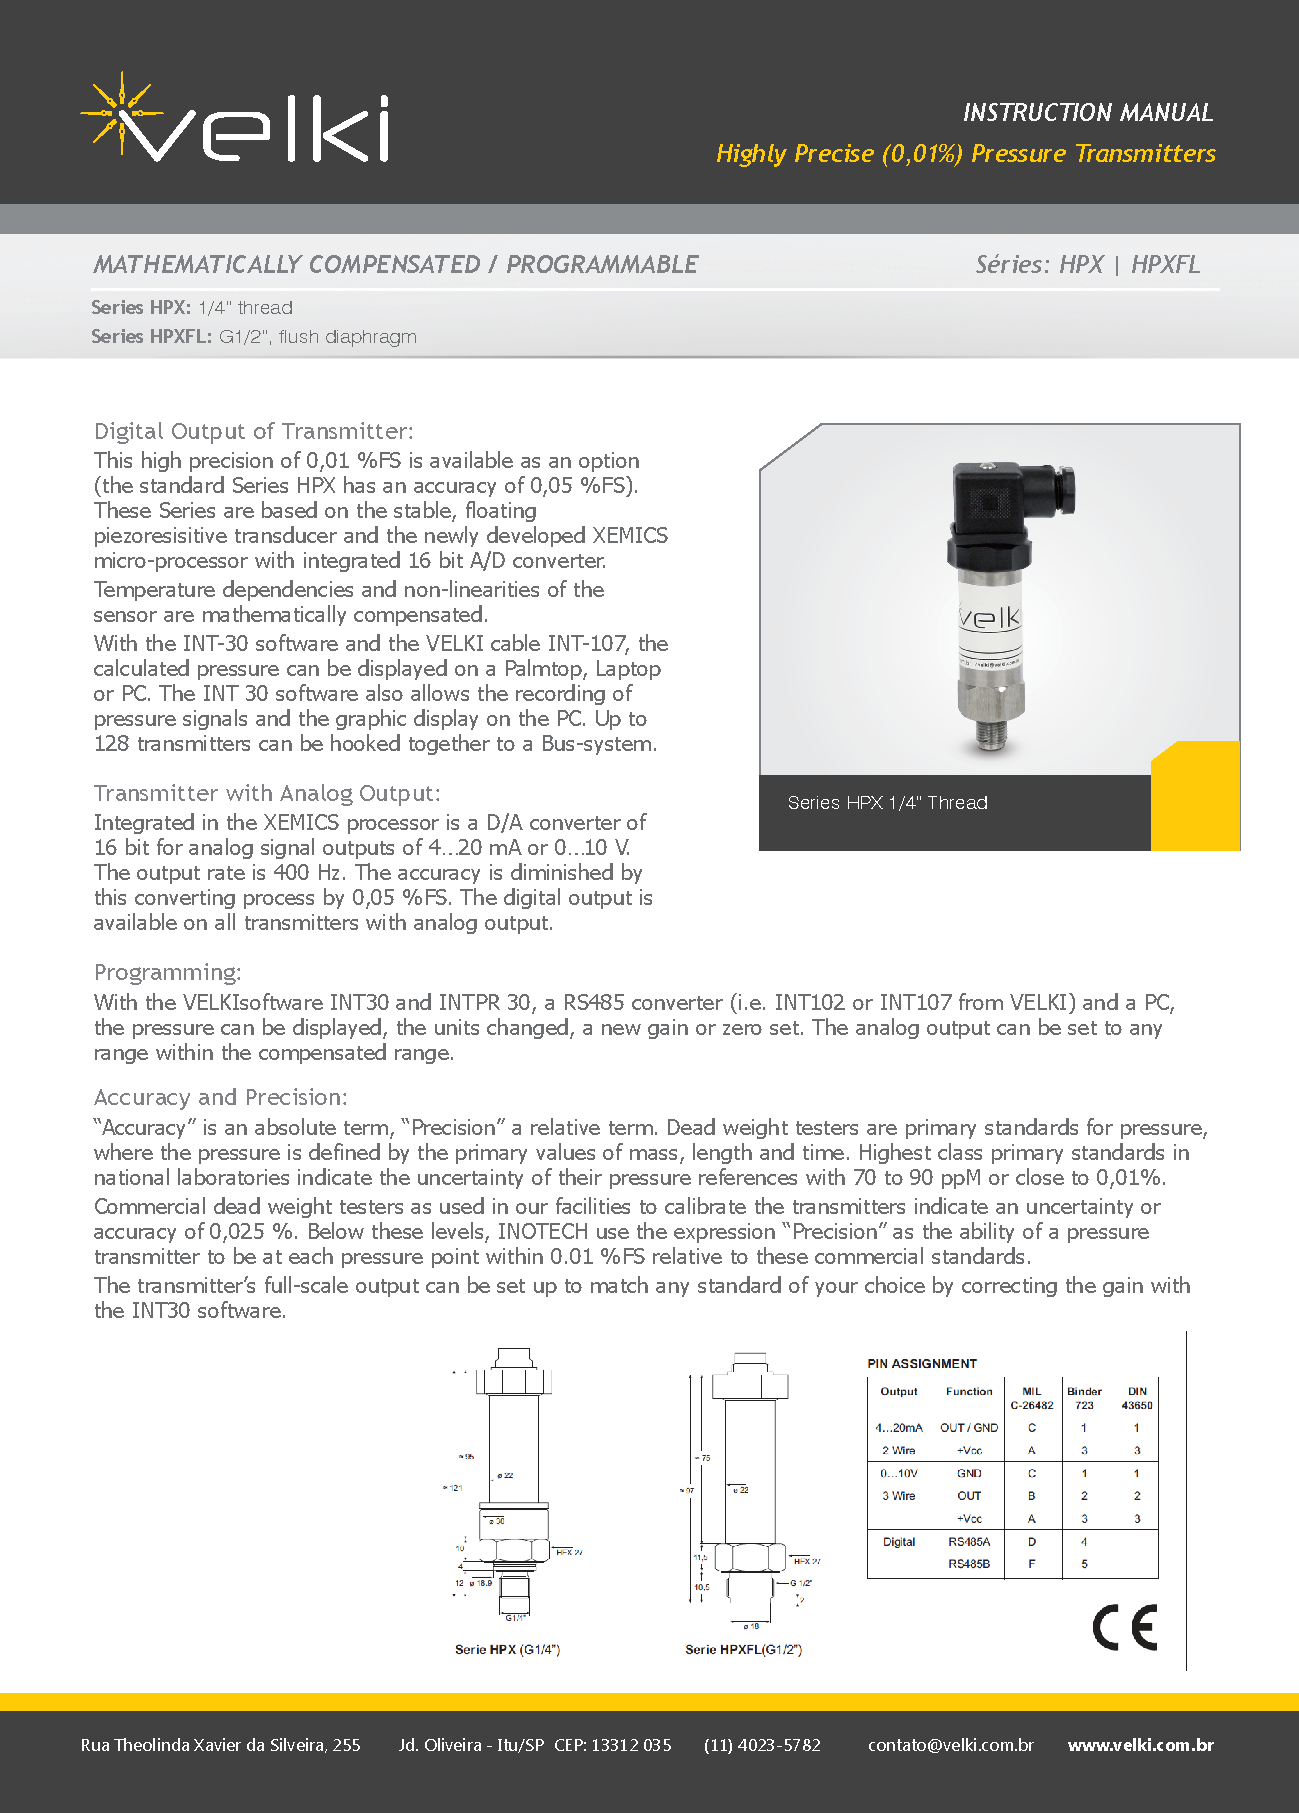
\includegraphics[width=1\columnwidth]{figs/datasheets/profundimetro.pdf}
\includepdf[pages={2-},width=1\columnwidth,pagecommand=\thispagestyle{plain}]{figs/datasheets/profundimetro.pdf}
\section{Pinagem}
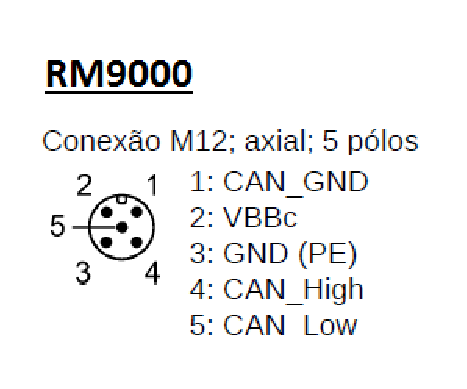
\includegraphics[width=1\columnwidth]{figs/datasheets/pinout.pdf}
\includepdf[pages={2-},width=1\columnwidth,pagecommand=\thispagestyle{plain}]{figs/datasheets/pinout.pdf}

